\chapter{Amminoacidi e proteine}
\section{Amminoacidi}
Un \textbf{amminoacido} è un composto che contiene sia un gruppo carbossilico che uno amminico. Gli amminoacidi che formano le proteine sono gli \textbf{\iupac{\a-amminoacidi}}, in quanto il gruppo amminico si trova sul carbonio adiacente al gruppo carbossilico.

\begin{figure}[H]
	\centering
	\begin{subfigure}{0.4\textwidth}
		\centering
		\chemfig{R-[:-30]CH(-[2,0.4,,,draw=none]{\color{blue}\scriptstyle\a})(-[6]NH_2)-[:30]C(=[2]O)(-[:-30]OH)}
		\caption{Forma non ionizzata}\label{fig:amminoacido}
	\end{subfigure}
	\begin{subfigure}{0.4\textwidth}
		\centering
		\chemfig{R-[:-30]CH(-[2,0.4,,,draw=none]{\color{blue}\scriptstyle\a})(-[6]\charge{135:3pt=\chargeColor{+}}{N}H_3)-[:30]C(=[2]O)(-[:-30]\charge{45:3pt=\chargeColor{-}}{O})}
		\caption{Forma dipolare (zwitterione)}\label{fig:zwitterione}
	\end{subfigure}
	\caption{Struttura di un amminoacido}
\end{figure}

Nonostante la~\autoref{fig:amminoacido} rappresenti l'amminoacido in forma non polare, in realtà l'amminoacido lo troviamo in forma dipolare. Questa forma viene chiamata col nome di \textbf{zwitterione} (\autoref{fig:zwitterione}). I zwitterioni hanno carina netta uguale a zero perché contengono sia una carica positiva che una negativa.

Tutti gli amminoacidi, tranne la glicina, hanno uno stereocentro questo li fa diventare dei composti chirali. In natura, gli \iupac{\a-amminoacidi} fanno parte della serie \L, rispetto alla gliceraldeide\footnote{Il metodo per dare la serie agli amminoacidi è uguale a quello che si usa per i carboidrati (\autoref{sec:chiralitaMonosaccaridi} a pagina~\pageref{sec:chiralitaMonosaccaridi})}.

La~\autoref{tab:amminoacidi_P1} riporta i nomi, le formule e le abbreviazioni standard a una e a tre lettere per i 20 \iupac{\L-amminoacidi} comunemente reperibili nelle proteine.
\begin{table}[H]
	\centering
	\setchemfig{
		atom sep=1.3em
	}
	\setlength\belowrulesep{10pt}
	\setlength\aboverulesep{10pt}
	\newcommand{\tab}[2]{\renewcommand{\arraystretch}{1.3}\begin{tabular}{c}\scshape#1\\#2\end{tabular}}
	\begin{NiceTabular}{r @{}>{\quad\footnotesize\bfseries\centering}m{4cm} r @{}>{\quad\footnotesize\bfseries\scshape}l}
		\toprule
		\Block{1-4}{Catene laterali non polari}                   &                           &               &                             \\
		\midrule
		\alanina                                                  & \tab{alanina}{Ala (A)}    & \fenilalanina & \tab{fenilalanina}{Phe (F)} \\
		\Block[r]{}<\renewcommand{\arraystretch}{4}>{\glicina}    & \tab{glicina}{Gly (G)}    & \prolina      & \tab{prolina}{Pro (P)}      \\
		\isoleucina                                               & \tab{isoleucina}{Ile (I)} & \triptofano   & \tab{triptofano}{Trp (W)}   \\
		\leucina                                                  & \tab{leucina}{Leu (L)}    & \valina       & \tab{valina}{Val (V)}       \\
		\Block[r]{}<\renewcommand{\arraystretch}{4}>{\metionina}  & \tab{metionina}{Met (M)}  &               &                             \\
		\midrule
		\Block{1-4}{Catene laterali polari}                       &                           &               &                             \\
		\midrule
		\asparagina                                               & \tab{asparagina}{Asn (N)} & \serina       & \tab{serina}{Ser (S)}       \\
		\Block[r]{}<\renewcommand{\arraystretch}{4}>{\glutammina} & \tab{glutammina}{Gln (Q)} & \tronina      & \tab{treonina}{Thr (T)}     \\
		\bottomrule
	\end{NiceTabular}
	\caption{Nomi e formule degli \iupac{\L-\a-amminoacidi}}\label{tab:amminoacidi_P1}
\end{table}
\begin{table}[H]
	\centering
	\setchemfig{
		atom sep=1.3em
	}
	\setlength\belowrulesep{10pt}
	\setlength\aboverulesep{10pt}
	\newcommand{\tab}[2]{\renewcommand{\arraystretch}{1.3}\begin{tabular}{c}\scshape#1\\#2\end{tabular}}
	\begin{NiceTabular}{r @{}>{\quad\footnotesize\bfseries\scshape\centering}m{4cm} r @{}>{\footnotesize\quad\bfseries\scshape}l}
		\toprule
		\Block{1-2}{Catene laterali acide} &                               & \Block{1-2}{Catene laterali acide} &                         \\
		\midrule
		\acidoAspartico                    & \tab{Ac. aspartico}{Asp (D)}  & \arginina                          & \tab{arginina}{Arg (R)} \\
		\acidoGlutammico                   & \tab{Ac. glutammico}{Glu (E)} & \istidina                          & \tab{istidina}{His (H)} \\
		\cisteina                          & \tab{cisteina}{Cys (C)}       & \lisina                            & \tab{lisina}{Lys (K)}   \\
		\tirosina                          & \tab{tirosina}{Tyr (Y)}       &                                    &                         \\
		\bottomrule
	\end{NiceTabular}
	\caption{Nomi e formule degli \iupac{\L-\a-amminoacidi}}\label{tab:amminoacidi_P2}
\end{table}

\section{Proprietà acido-base degli amminoacidi}
Gli amminoacidi sono acidi deboli poliprotici a causa della presenza dei gruppi \ch{-COOH} e \ch{-NH3^{+}}, per questo motivo si comportano da \textit{anfoteri}.

\subsection{Acidità e basicità dei gruppi \texorpdfstring{\a}{α}}
Il valore della \pKa\ di un gruppo \iupac{\a-carbossilico} in un amminoacido protonato è di 2,19. Questo valore confrontato con quello di altri acidi carbossilici, che è di circa 4,76, è molto minore. Questo abbassamento di \pKa\ viene giustificato dall'effetto induttivo del gruppo ammonio adiacente.
L'effetto induttivo del gruppo ammonio influenza anche i gruppi \iupac{\b-COOH} dell'acido aspartico (\pKa\ 3,86) e del \iupac{\g-COOH} dell'acido glutammico (\pKa\ 4,07).

Anche il valore della \pKa\ del gruppo \iupac{\a-ammonio} viene influenzato dal gruppo carbossilico, il quale si abbassa da 10,60 a 9,47. Di conseguenza, il gruppo \iupac{\a-ammonio} risulta più acido di un'ammina primaria alifatica.

\subsection{Titolazione degli amminoacidi}
I valori di \pKa\ degli amminoacidi sono stati ottenuti tramite titolazione acido-base, misurando il \pH\ della soluzione in funzione della base aggiunta.

\subimport*{../../../grafici/}{TitolazioneAlanina.tex}

Il comportamento degli amminoacidi quando vengono titolati è illustrato con i seguenti equilibri:
\setchemfig{arrow label sep=7pt}
\begin{reaction}
	\AddRxnDesc{Titolazione amminoacido}
	\chemfig{R-[:-30]CH(-[6]\charge{135:3pt=\chargeColor{+}}{N}H_3)-[:30]C(=[2]O)(-[:-30]OH)}
	\arrow{<=>[\chemfig{H\charge{45:3pt=\chargeColor{-}}{O}}][\chemfig{\charge{30:3pt=\chargeColor{+}}{H}}]}
	\chemfig{R-[:-30]CH(-[6]\charge{135:3pt=\chargeColor{+}}{N}H_3)-[:30]C(=[2]O)(-[:-30]\charge{45:3pt=\chargeColor{-}}{O})}
	\arrow{<=>[\chemfig{H\charge{45:3pt=\chargeColor{-}}{O}}][\chemfig{\charge{30:3pt=\chargeColor{+}}{H}}]}
	\chemfig{R-[:-30]CH(-[6]NH_2)-[:30]C(=[2]O)(-[:-30]\charge{45:3pt=\chargeColor{-}}{O})}
\end{reaction}

Quando un amminoacido, un polipeptide o una proteina hanno una carica netta uguale a 0 a un determinato \pH\ questo valore prende il nome di \textbf{punto isoelettrico (pI)}. Questo valore varia a seconda dell'amminoacido.

Sapendo questo, possiamo separare una soluzione di amminoacidi applicando un potenziale elettrico a un determinato \pH, questo farà migrare gli amminoacidi verso l'elettrodo con carica inversa alla loro mentre gli amminoacidi che si trovano nel loro punto isoelettrico rimarranno fermi. Questo processo prende il nome \textbf{elettroforesi}.

\section{Polipeptidi}
Gli amminoacidi si concatenano nei peptidi e nelle proteine tramite legami ammidici chiamati \textbf{legami peptidici} da Fischer. Una molecola formata da due amminoacidi viene chiamata \textbf{dipeptide}.

\begin{figure}[H]
	\centering

	\chemfig{H_3-[,0.5,,,draw=none]@{N}\charge{50:3pt=\chargeColor{+}}{N}-[:-30]CH(-[6]R)-[:30]C(=[2]O)-[@{L}:-30]NH-[:30]CH(-[2]R')-[:-30]@{C}C(=[6]O)-[:30]\charge{45:3pt=\chargeColor{-}}{O}}

	\chemmove[transform shape,every node/.style={fill=white}]{
		\draw[draw=none] (L) -- +(0,1.3) coordinate (n1);
		\draw[-,dashed] (n1) -- +(0,-2.8) coordinate (n2);
		\draw[latex-latex,shorten <=3pt, shorten >= 1pt,anchor=mid,blue] (n2) -- node{aa$_2$} +(4,0);
		\draw[latex-latex,shorten <=3pt, shorten >= 1pt,anchor=mid,blue] (n2) -- node{aa$_1$} +(-3,0);
		\node[font=\scriptsize,text=purple] (pep) at (1,3) {legame peptidico};
		\draw[-latex,shorten >= 4pt,color=purple] (pep) .. controls +(225:2cm) and +(45:2cm) ..  (L);
		\node[font=\scriptsize,text=purple] (pep) at (4,0) {aa C-terminle};
		\draw[-latex,shorten >= 4pt,color=purple] (pep.160) .. controls +(135:1.5cm) and +(-45:1.7cm) ..  (C);
		\node[font=\scriptsize,text=purple] (pep) at (-4,2.5) {aa N-terminale};
		\draw[-latex,shorten >= 4pt,color=purple] (pep) .. controls +(-45:2cm) and +(135:2cm) ..  (N);
	}
\end{figure}

\NewChemIUPAC\C{\textit{C}}

Per convenzione, i polipeptidi vengono scritti a partire cominciando con il gruppo \ch{-NH_3-} libero e procedendo verso l'amminoacido con il gruppo \ch{-COO-}. L'amminoacido con il gruppo \ch{-NH_3-} libero è detto \textbf{amminoacido \iupac{\N-terminale}} mentre quello con il \ch{-COO-} libero viene detto \textbf{amminoacido \iupac{\C-terminale}}.

\section{Le proteine e loro strutture}
La struttura delle proteine è molto complessa e può essere definita in quattro livelli che vengono chiamati:
\begin{itemize}
	\item \textbf{struttura primaria}, è la sequenza degli amminoacidi nella catena
	\item \textbf{struttura secondaria}, comprende le conformazioni assunte dai vari tratti della catena
	\item \textbf{struttura terziaria}, è la struttura tridimensionale complessiva
	\item \textbf{struttura quaternaria}, si riferisce alle proteine formate da più catene e definisce come quest'ultime interagiscono tra di loro
\end{itemize}

\subsection{Struttura primaria}
La \textbf{struttura primaria} è la sequenza di amminoacidi che compongono la proteina, uniti tramite legami peptidici.

La sequenza di amminoacidi che compone la catena polipeptidica è molto importante perché determina la struttura tridimensionale della proteina.

\subsection{Struttura secondaria}
\subsubsection{Geometria del legame peptidico}
\noindent Le principali caratteristiche della struttura dei peptidi sono:
\begin{enumerate}
	\item Il gruppo ammidico giace sul piano, contenente il carbonio carbonilico, l'azoto e i quattro atomi a essi legati
	\item Il legame \ch{C-N} ha un parziale carattere di doppio legame
	\item Non è detto che solo perché i gruppi ammidici sono planari devono essere sullo stesso piano di quelli adiacenti, in ragione della libera rotazione intorno ad altri legami semplici. Infatti il gruppo \ch{-CHR} ha libera rotazione.
\end{enumerate}

\subsubsection{L'\texorpdfstring{\a}{α}-elica e il foglietto \texorpdfstring{\b}{β}-ripiegato}
\begin{minipage}{.4\textwidth}
	\begin{figure}[H]
		\centering
		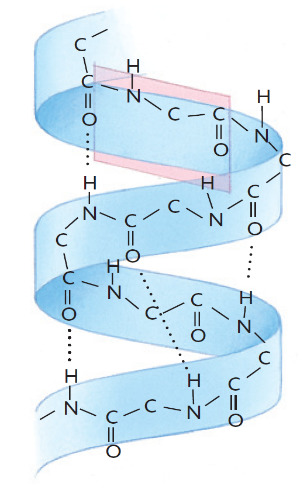
\includegraphics{immagini/alpha-elica.jpg}
		\vspace{10pt}
	\end{figure}
\end{minipage}
\begin{minipage}{.55\textwidth}
	La \textbf{struttura ad \iupac{\a-elica}} è destrorsa e gli amminoacidi si avvolgono attorno ad un asse centrale con i gruppi R in catena laterale puntano verso l'esterno. Ponendo in alto l’amminoacido \iupac{\N-terminale}, i legami peptidici ruotano in modo da rivolgere tutti i carbonili \ch{C=O} in basso per formare legami idrogeno con i gruppi \ch{N-H} sottostanti. Per ogni giro dell'elica ci sono 3,6 amminoacidi.
\end{minipage}

\begin{minipage}{.55\textwidth}
	La \textbf{struttura a foglietto \iupac{\b-ripiegato}} in catene adiacenti che si sviluppano in direzioni opposte tenute assieme tramite legami a idrogeno. Differentemente dalla disposizione nell’\iupac{\a-elica}, i gruppi \ch{N-H} e \ch{C=O} giacciono nel piano del foglietto e sono perpendicolari all’asse lungo del foglietto. Il gruppo \ch{C=O} di ciascun legame peptidico forma un legame idrogeno con il gruppo \ch{N-H} di un legame peptidico di una catena adiacente. I gruppi R su una qualunque catena si alternano sopra e sotto il piano del foglietto.
\end{minipage}
\begin{minipage}{.4\textwidth}
	\begin{figure}[H]
		\centering
		\vspace{-10pt}
		% TODO: fare tu l'immagine
		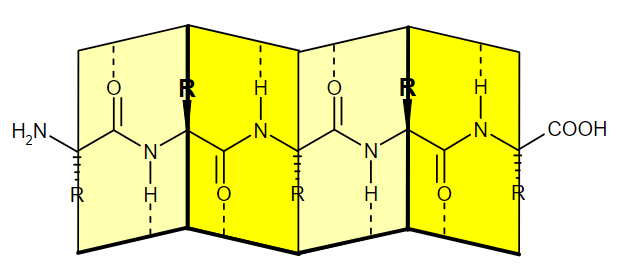
\includegraphics[scale=0.5]{immagini/Code_IL8tmGoF4t.png}
	\end{figure}
\end{minipage}

\subsection{Struttura terziaria}
La \textbf{struttura terziaria} è rappresentata dalla configurazione tridimensionale che la catena polipeptidica assume nell'ambiente in cui si trova. La struttura terziaria è stabilizzata da legami idrogeno e ponti disolfuro.


\paragraph{Legame disolfuro}\mbox{}\\
I \textbf{legami disolfuro} (\autoref{par:disolfuri}) si formano tra due cisteine per ossidazione dei loro gruppi tiolici. Se le due unità si trovano sulla stessa catena, il legame provocherà la formazione di ansa. Se invece, le due unità si trovano su due catene diverse, il legame collegherà le due catene.

\begin{reaction}
	\AddRxnDesc{Formazione del legame disolfuro tra due amminoacidi}
	\arrow{0}[,0]
	\subscheme[-90]{
	\chemfig{-[:30,,,,dashed]\chemabove{N}{H}-[:-30](-[6]@{S1}-[:-30]SH)-[:30](=[2]O)-[:-30]\chembelow{N}{H}-[:30,,,,dashed]}
	\arrow{0}[,0.2]
	\chemfig{-[:-30,,,,dashed]\chembelow{N}{H}-[:30](-[2]@{S2}-[:30]SH)-[:-30](=[6]O)-[:30]\chemabove{N}{H}-[:-30,,,,dashed]}
	}
	\arrow{<=>[ossidazione][riduzione]}[,2]
	\chemfig{-[:30,,,,dashed]\chemabove{N}{H}-[:-30](-[6]-[:-30]S-[@{Sl}6]S-[:210]-[6](-[:210]\chembelow{N}{H}-[:150,,,,dashed])(-[:-30](=[6]O)-[:30]\chemabove{N}{H}-[:-30,,,,dashed]))-[:30](=[2]O)-[:-30]\chembelow{N}{H}-[:30,,,,dashed]}
	\chemmove[green!60!black!70]{
		\node[xshift=-2cm,yshift=-8pt,align=left,font=\scriptsize] (text) at ($(S1)!0.5!(S2)$) {catene laterali\\ della cisteina};
		\draw[shorten >=6pt,] (text.east) -- (S1);
		\draw[shorten >=6pt,] (text.east) -- (S2);
		\draw[latex-,shorten >=2pt,shorten <= 2pt] (Sl) -- +(.5,.5) node[above right] {\scriptsize legame disolfuro};
	}
\end{reaction}

\subsection{Struttura quaternaria}
La \textbf{struttura quaternaria} è quella che deriva dall'associazione di due o più unità polipeptidiche, unite tra loro da legami deboli (e a volte ponti disolfuro) in un modo molto specifico.